\newpage
\section{SLIP}

Giả sử các bạn đang làm về ứng dụng về cảm biến có truyền dữ liệu từ MCU đọc cảm biến về MCU trung tâm. Như khung truyền dữ liện biến evn\_t như đã trình bày ở chương trước, biến này có độ dài 4 byte, sau khi nhận đủ 4 byte thì MCU trung tâm bắt đầu xử lí. Vậy đặt trường hợp MCU trung tâm không biết biến truyền về có bao nhiêu byte thì bạn làm thế nào?

Trong các dự án thực tế, dữ liệu trao đổi giữa 2 MCU thường rất đa dạng, khác nhau về mục đích của dữ liệu, tính chất, độ dài, số lượng\dots Ví dụ về các mục đích truyền: để truyền data như các thông tin về môi trường, để điều khiển như bật tắt một bóng đèn, để cấu hình, như việc MCU trung tâm thay đổi mật khẩu mã hóa và truyền thông tin này đến các thiết bị khác\dots

Thế nên việc biết trước độ dài dữ liệu là dường như không thể. Cố gắng quy định độ dài mỗi lần truyền sẽ làm mất đi tính linh hoạt của chương trình. 

SLIP sinh ra để giải quyết vấn đề này.

Ý tưởng đằng sau đó là có một byte đánh dấu kết thúc chuỗi với giá trị là 0xC0 (gọi tắt là END), khi MCU nhận được trong chuỗi data có giá trị này thì tiến hành xử lí dữ liệu nhận được trước đó.

\begin{wrapfigure}{l}{0.5\textwidth}
	\centering
    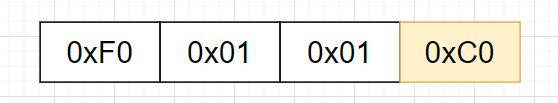
\includegraphics[width=0.4\textwidth]{SlipEnd.PNG}
\caption{Slipe End}
\end{wrapfigure}

Nhưng vấn đề dữ liệu là một số bất kì, trong dữ liệu truyền về đôi khi sẽ có giá trị END và MCU nhận sẽ hiểu lầm rằng đã nhận được đủ dữ liệu và tiến hành xử lí. Điều này chắc chắn sẽ gây lỗi trong chương trình.

\begin{wrapfigure}{l}{0.5\textwidth}
	\centering
    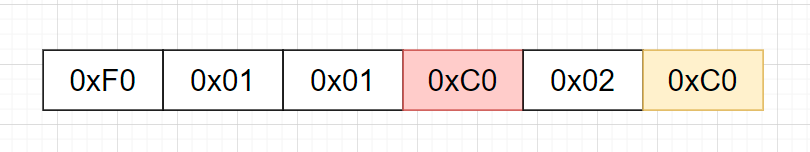
\includegraphics[width=0.5\textwidth]{SlipEndError.PNG}
\caption{Slipe End Error}
\end{wrapfigure}

\begin{wrapfigure}{l}{0.5\textwidth}
	\centering
    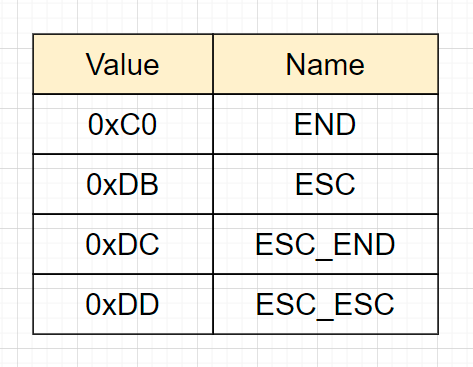
\includegraphics[width=0.4\textwidth]{SlipTable.PNG}
    \caption{Slip table}
    \label{SlipTable}
\end{wrapfigure}

Để giải quyết vấn đề này, người ta tiến hành mã hóa dữ liệu truyền, sao cho trong dữ liệu đó không xuất hiện giá trị END nữa. Cách mã hóa được thực hiện như sau: quy định thêm 3 giá trị đặc biệt ESC, ESC\_END, ESC\_ESC có giá trị như trong hình \ref{SlipTable}.

Nếu trong dữ liệu có giá trị END, nó sẽ được thay bằng chuỗi 2 giá trị ESC và ESC\_END. 

Nếu dữ liệu có ESC, nó sẽ được chèn thêm ESC\_ESC ngay sau đó, xem hình \ref{EncodeSlip}.

Ở chiều ngược lại khi giải mã, MCU nhận được END sẽ biết là chuỗi dữ liệu truyền đã xong, nhận được ESC sẽ biết trong dữ liệu sắp nhận được có giá trị đặc biệt, hoặc là trùng với END hoặc trùng với chính ESC. Nếu ngay sau đó là ESC\_END, nó sẽ thêm biến END vào dữ liệu, nếu là ESC\_ESC, nó sẽ thêm ESC vào dữ liệu nhận được.

 Việc mã hóa trên đã đảm bảo trong dữ truyền không xuất hiện END trên đường truyền, và giải mã đúng dữ liệu khi đã nhận được dù nó có kí tự END hay không, nhưng đồng thời làm tăng kích thước dữ liệu trên đường truyền và tăng thời gian xử lí của MCU. Tuy nhiên, điều này là không đáng kể để đổi lại tính linh hoạt khi hoạt động của chương trình.

\begin{figure}[h!]
    \centering
    \subfloat[Encode END]{
        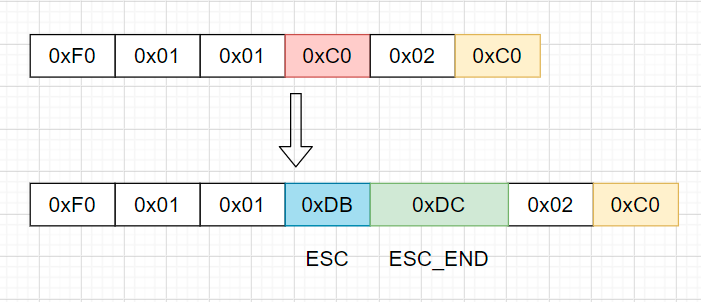
\includegraphics[width=0.5\textwidth]{ESCEND.PNG}
    }
    \subfloat[Encode ESC]{
        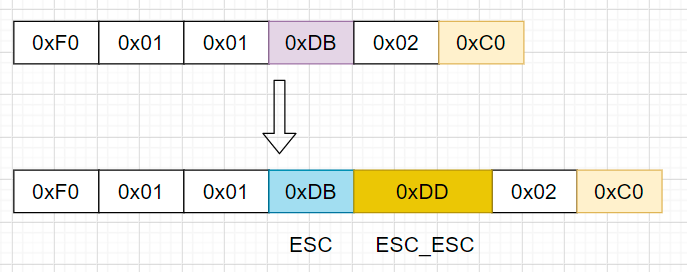
\includegraphics[width=0.5\textwidth]{ESCESC.PNG}
    }
    \caption{Encode Slip}
    \label{EncodeSlip}
\end{figure}
